\section{Umsetzung des Prototypen emoTrix}
In diesem Abschnitt wird die Umsetzung des Prototyps beschrieben. Dabei werden neben dem Programmcode auch aufgetretene Probleme beschrieben.
\subsection{MockUps}
\subsectionauthor{Torben Brenner}
Bevor wir mit der Arbeit an dem Prototypen begonnen haben, diskutierten wir zuerst das Design der einzelnen Komponenten der Anwendung. Wir einigten uns darauf, dass die Übersicht über alle Teile des Prototypen auf der Hauptseite des Startbildschirms sein soll (siehe \ref{img:Mockup-Home}).
\begin{figure}[h]
	\centering
	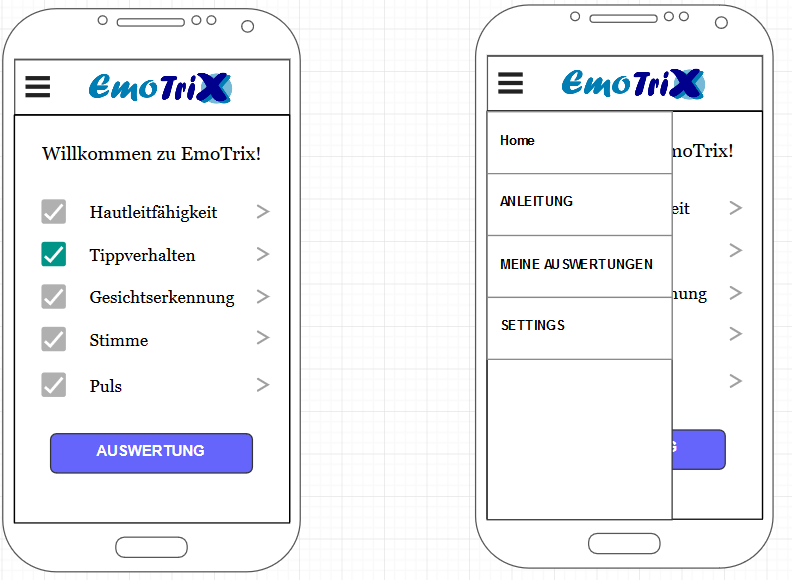
\includegraphics[width=10cm]{Bilder/Mockup-Home.png}
	\label{img:Mockup-Home}
	\caption[Mockup - Homescreen(links) und Menü(rechts)]{Mockup - Homescreen(links) und Menü(rechts)}
\end{figure}%
Wie auf der Grafik zu sehen ist, sind für die fertige Anwendung 5 verschiedene Arten von Tests vorgesehen. Die dazugehörigen Anwendungsabschnitte sollen von der Startseite, durch anklicken des Testnamens aufgerufen werden können und dann ausgeführt werden können. Durch das Berühren des Auswertungsknopfes soll es möglich sein, eine Analyse der verschiedenen Testergebnisse durchzuführen. Diese gibt dann als Ergebnis eine Übersicht heraus, welche Emotionen wie wahrscheinlich sind. Eine Übersicht der bereits durchgeführten Auswertungen soll über das Menü (siehe \ref{img:Mockup-Home} rechts) erreichbar sein. In der Anleitung(ebenfalls über das Menü erreichbar) sollen sich Beschreibungen zur Durchführung der einzelnen Tests befinden.\newline
Im folgenden sollen neben den einzelnen Test Seiten auch die Auswertungsseite genauer beschrieben werden.
\subsubsection{Hautleitfähigkeit}
\subsubsectionauthor{Torben Brenner}
\textbf{Todo:}
\subsubsection{Tippverhalten}
\subsubsectionauthor{Torben Brenner}
Beim Test des Tippverhaltens, ist es angedacht das der Nutzer eine Zeit angibt in der die Anwendung seine Tastatureingaben beobachten darf. Diese Zeit soll in Minuten angegeben werden und läuft intern als Timer ab während der Nutzer im Vordergrund mit anderen Anwendungen, wie z. Bsp. dem Internet Browser oder unterschiedlichen Messenger Applikationen agiert. Dies benötigt ausdrücklich die Erlaubnis, da es ansonsten möglich wäre Passwörter und sonstiges mit zu lesen. 
\begin{figure}[h]
	\centering
	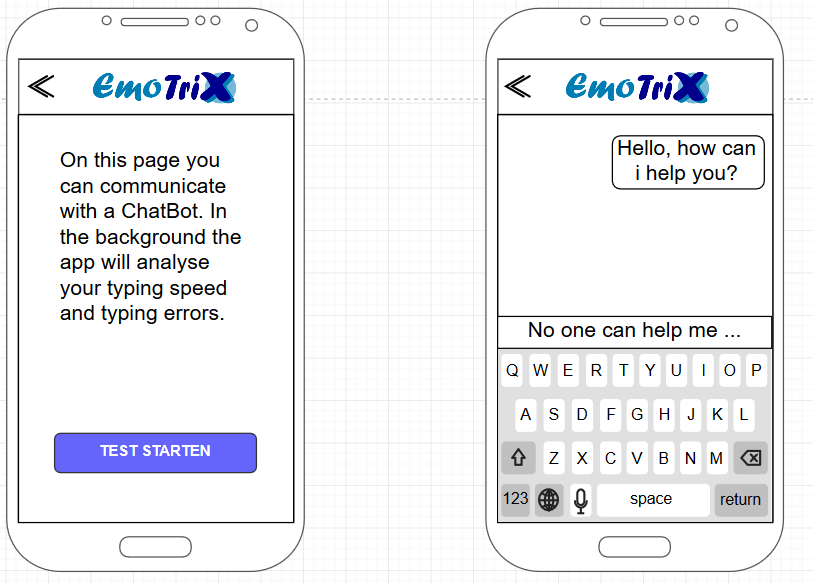
\includegraphics[width=10cm]{Bilder/Mockup-Tippverhalten.png}
	\label{img:Mockup-Tippverhalten}
	\caption[Mockup - Tippverhalten Test starten(links) und Test ergebnis(rechts)]{Mockup - Tippverhalten Test starten(links) und Test ergebnis(rechts)}
\end{figure}%
Auf der Ergebnisseite soll dem Nutzer dann die Möglichkeit geboten werden, sich die Erfassten Tastatureingaben anzeigen zu lassen. Hierfür wäre z. Bsp. ein Zeitstrahl eine gute Lösung, da Alle eingaben untereinander vermutlich zu viel Text sind und das Ergebnis unübersichtlich werden lassen würden. 
\subsubsection{Gesichtserkennung}
\subsubsectionauthor{Torben Brenner}
Bei der Gesichtserkennung wird der Nutzer von der Anwendung dazu aufgefordert, die Kamera zu starten und daraufhin ein Bild mit dieser zu machen. Die Anwendung analysiert dann das Bild mithilfe der im Konzept beschriebenen Methoden. Auf der Ergebnisseite wird dem Nutzer daraufhin das Bild zusammen mit einer Auflistung der Ermittelten Wahrscheinlichkeiten für die Unterschiedlichen Emotionen ausgegeben.
\begin{figure}[h]
	\centering
	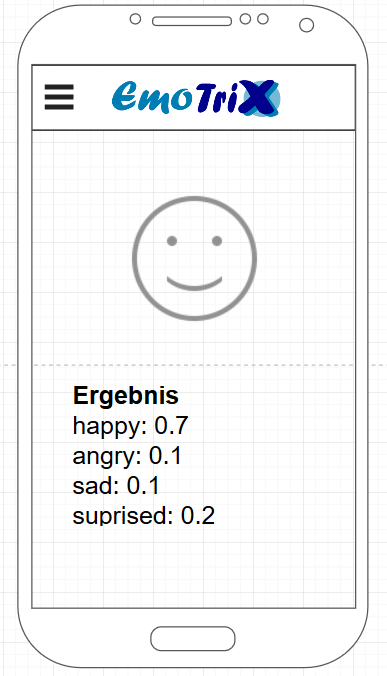
\includegraphics[width=4cm]{Bilder/Mockup-Gesichtserkennung.png}
	\label{img:Mockup-Gesichtserkennung}
	\caption[Mockup - Gesichtserkennung Ergebnisseite]{Mockup - Gesichtserkennung Ergebnisseite}
\end{figure} \newpage
\subsubsection{Auswertung}
\subsubsectionauthor{Torben Brenner}
Auf dem folgenden Bild ist die Auswertungsseite zu sehen. 
\begin{figure}[h]
	\centering
	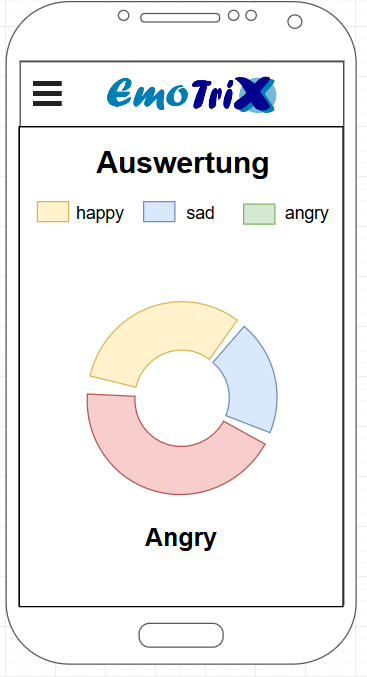
\includegraphics[width=4cm]{Bilder/Mockup-Auswertung.png}
	\label{img:Mockup-Auswertung}
	\caption[Mockup - Auswertung]{Mockup - Auswertung}
\end{figure} \newline
Die Seite enthält sowohl eine Legende, die angibt welche Farbe welche Emotion repräsentiert, als auch ein Auswertungsergebnis in Form eines Kreisdiagramms. Unter dem Diagramm soll der Nutzer einen Text angezeigt bekommen, welche Emotion aktuell überwiegt.
\subsection{Umsetzung der Backendlogik}
\subsectionauthor{Torben Brenner}
Wie im Konzept beschrieben besteht das Backend der Anwendung aus den Klassen \textit{Decider, CausalityRule} und der Abstrakten Klasse \textit{Sensor}. Im folgenden wird die Umsetzung der einzelnen Klassen beschrieben.\newline
Die Klasse \textit{Sensor} wurde als Abstrakte Klasse umgesetzt. Dies ermöglicht es dem Entwickler, für jeden Test eine Klasse zu implementieren die von der Architektur verstanden wird und in der er die im Test ermittelten Daten auswerten kann. Die Implementation der \textit{Sensor} Klasse sieht folgendermaßen aus: 
\begin{lstlisting}[caption={abstrakte Klasse Sensor},language=JavaScript]
export abstract class Sensor{

	constructor(public decider: Decider){};

	// this forces the specific sensor evaluators to implement this method
	abstract mapper(data: any): IndicatorScore[]; 

	onSensorData(data: any) {
		let indicatorScores = this.mapper(data)
		this.decider.addIndicatorScores(indicatorScores);
	}

}
\end{lstlisting}
Der Konstruktor der Klasse empfängt eine Instanz der Klasse \textit{Decider}, die wie im Konzept beschrieben ein Singleton ist. Die Funktion \textit{onSensorData} wird von den Subklassen aufgerufen, sobald Daten empfangen wurden und stellt die Logik der Sensor Klasse dar. Zuerst wird bei Empfang der Daten, das von erbenden Klassen definierte \textit{Mapping} auf die Daten ausgeführt. Danach werden die Daten dem \textit{Decider} hinzugefügt, welcher diese dann im späteren Verlauf verarbeiten kann(Vgl. \ref{img:Ablauf Erstellung Indicatorscores}). Durch das Schlüsselwort \textit{abstract} wird bei der Funktion \textit{mapper} gekennzeichnet, dass dieser von den erbenden Klassen implementiert werden soll. Die Abstrakte Klasse definiert in diesem Fall nur, dass der Mapper aus den Daten des Sensors eine Liste von \textit{IndicatorScores} erzeugen muss. Ein \textit{IndicatorScores} besteht dabei aus einem \textit{indicator} und einem \textit{score}. Der Score ist als nummerischer Wert definiert und für die Indicator wurde ein eigener Typ definiert. Dieser Typ ermöglicht es, eine einfache Prüfung der Werte gegenüber dem Typ String und bestimmten Werten durchzuführen. Erlaubte Werte für den Typ Indicator sind zum Beispiel: \textit{"stress"} oder \textit{"angryIndicator"}.\newline
Wie im Konzept beschrieben, verwaltet die Klasse \textit{Decider} alle \textit{IndicatorScores}. Um sicherzustellen, dass die Daten nach Zeitpunkt sortiert gespeichert werden, ermittelt die Methode \textit{addIndicatorScores} erst einen Zeitpunkt und speichert danach die Daten in einer List von Objekten, welche den Zeitpunkt und die dazu gehörige Liste von \textit{IndicatorScores} enthalten. Dadurch können Sensoren die \textit{IndicatorScores} einfach auf diese Liste pushen, ohne Gefahr zu laufen sich gegenseitig zu überschreiben.\newline
Um die Auswertung der Daten zu ermöglichen, greift die Klasse \textit{Decider} außerdem auf eine Liste von Kausalitätsregeln zu. Diese können mit der Klasse \textit{CausalityRule} definiert werden.
Der Konstruktor dieser Klasse nimmt zwei Parameter entgegen. Der Parameter \textit{condition} repräsentiert eine Bedingung, welche eintreten muss sodass die Kausalitätsregel angewandt wird. Die Bedingung wurde innerhalb der Anwendung durch einen Typ umgesetzt. Der Typ prüft dabei auf eine Funktion, die entweder einen oder zwei \textit{indicator} als Parameter entgegennimmt, und als Rückgabewert wahr oder falsch zurückgibt. 
\begin{lstlisting}[caption={Typ condition}, language=JavaScript]
	type Condition = (indicatorA: IndicatorScore, indicatorB?: IndicatorScore) => boolean;
\end{lstlisting}
Das bedeutet, dass die Bedingung vom Entwickler frei über die \textit{IndicatorScores} definiert werden kann. Der zweite Parameter der Anwendung repräsentiert die Auswirkungen der Kausalitätsregel beim eintreffen der Bedingung. Um diesen Parameter zu definieren wurde ebenfalls ein neuer Typ angelegt. Dieser prüft auf Funktionen, die eine Liste von \textit{EmotionScores} entgegen nehmen und eine solche auch wieder zurückgeben. Das bedeutet, dass in Funktionen dieser Art irgendeine Manipulation der \textit{EmotionScores} stattfinden muss. Der Parameter der Kausalitätsregel ist eine Liste solcher Funktionen. Mit diesen beiden Funktionen kann nun in der Klasse \textit{CausalityRule} eine neue Funktion definiert werden, die prüft ob eine Bedingung eingetroffen ist und in diesem Fall, alle Auswirkungen der Regel ausführt. 
\begin{lstlisting}[caption={execute Funktion der Klasse CausalityRule},language=JavaScript]

public execute(data : Array<EmotionScore>, indicatorScores: IndicatorScore[]) {
	indicatorScores.forEach((indicatorScore) =>{
		if(this.condition(indicatorScore)){
			this.effects.forEach((effect) => {
				data = effect(data);
			})
		}});
		return data;
	}
}

\end{lstlisting}
Diese Funktion kann nun von der Klasse \textit{Decider} ausgeführt werden.
\textbf{Hier wird in Kürze weitergeschrieben}
\subsection{Datenerfassung in Form von Emotionstests}
\subsubsection{Face-Test}
\subsubsection{GSR-Test}
\subsubsectionauthor{Lukas Seemann}
Die Erfassungsmöglichkeit mit der höchsten Priorität war die Messung der Hautleitfähigkeit mithilfe von EDA- beziehungsweise GSR-Sensoren. Da dies nicht mit im Smartphone enthaltenen Sensoren möglich war, wurde zusätzlich ein Arduino-Mikrocontroller benötigt, um die Messung durchzuführen. Zunächst wird die Entwicklung auf dem Arduino-Board mit allen zusätzlichen Modulen beschrieben. Im Anschluss daran wird thematisiert, wie das Arduino-Board mit der App verbunden wurde. \newline
Für das Projekt wurde ein Arduino UNO R3 Board verwendet. \footcite[Vgl.][]{Ard18} Dieser kann mit Stromzufuhr über ein Netzteil oder per USB betrieben werden. Als Sensor wurde ein GSR Sensor des Grove-Toolkits verwendet\footcite[Vgl.][]{Gro18}, der bereits in Abbildung 5 gezeigt wird. Am Sensor selbst werden die Elektroden für die Finger angebracht. Da ein handelsübliches Arduino UNO R3 Board nicht über den benötigten Anschluss für den Grove GSR-Sensor verfügt, muss zusätzlich noch ein Grove Base Shield angebracht werden. Dieses kann auf das Arduino Board aufgesteckt werden und erweitert es um viele verschiedene Anschlüsse, unter anderem für Sensoren.
\begin{figure}[h]
	\centering
	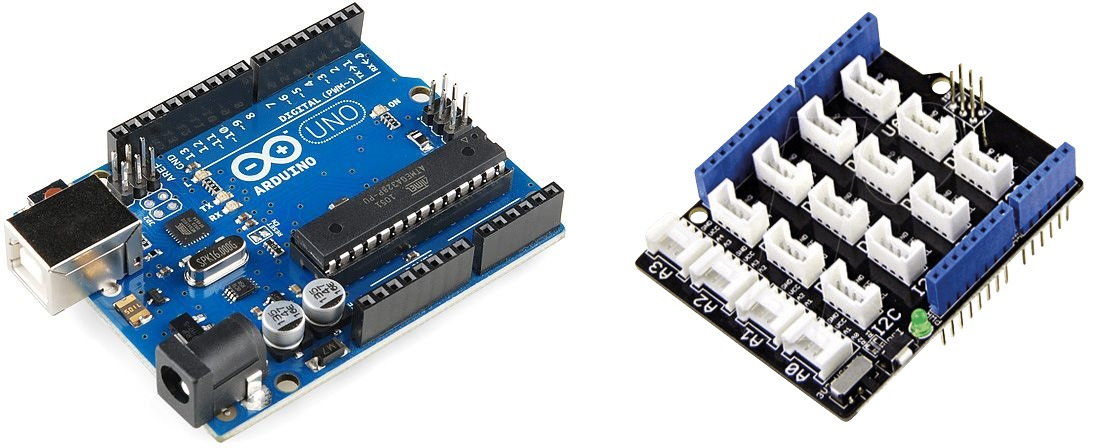
\includegraphics[width=16cm]{Bilder/arduino.jpg}
	\caption[Arduino UNO R3 (links) und Grove Base Shield]{Arduino UNO R3 (links) und Grove Base Shield\footnotemark}
\end{figure}%
\footcitetext[Bilder von:][]{Sou18, Rei18}
\newline \newline
Mit diesen Komponenten werden die vom Sensor zurückgelieferten Daten an den Arduino geleitet. Von dort aus müssen die Daten, an die mobile Applikation weitergeleitet werden. Aus diesem Grund muss an das Arduino Board ein Bluetooth-Modul angebracht werden, das Daten senden und empfangen kann. Das Empfangen von Daten ist notwendig, um die Messung zu Starten, wohingegen das Senden für die Übermittlung der Sensordaten benötigt wird. Heutige Smartphones verfügen meistens immer über eine Bluetooth-Schnittstelle, aus welchem Grund Bluetooth gut für die Übertragung geeignet ist. Eine weitere Möglichkeit wäre die Übertragung über WiFi gewesen. Das Arduino-Board wurde mit einem HC05-Bluetooth-Modul erweitert, welches Daten senden und empfangen kann. Dieses ist in Abbildung ? zu sehen.
\begin{figure}[h]
	\centering
	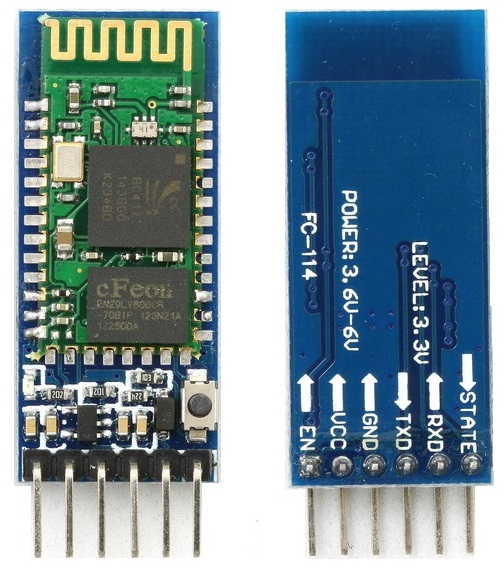
\includegraphics[width=7cm]{Bilder/hc05.jpg}
	\caption[HC-05-Bluetooth-Modul für Arduino]{HC-05-Bluetooth-Modul für Arduino\footnotemark}
\end{figure}%
\newline
Die Beschreibung der Entwicklungsarbeiten wird in zwei Teile aufgespalten. Der erste Teil ist der Quellcode des Arduinos, der zweite Teil die Entwicklung des Emotionstest in der emoTrix-App. \newline
In Listing ? ist der Quellcode des Arduinos abgebildet. In Zeile 1 wird die SofwareSerial-Bibliothek eingebunden, die eine Verwendung der Pins des Arduinos für verschiedene Module ermöglicht. In Zeile 2 wird dem Arduino mitgeteilt, dass auf den Pins 10 und 11 ein Bluetooth-Modul angeschlossen ist und eine Konstante (GSR) festgelegt, die auf den Anschluss A0 des Grove Shields verweist, an dem der GSR Sensor angeschlossen ist. \newline
Generell besteht der Programmcode des Arduinos immer aus zwei Bestandteilen: einem Setup-Block und einem Loop-Block. Der Setup-Block wird einmalig beim Einschalten des Arduinos ausgeführt. Danach wird der Loop-Block solange wiederholt, bis der Arduino ausgeschalten wird. \newline \newline 

\begin{lstlisting}[caption={Quellcode des Arduinos},style=Arduino]
#include <SoftwareSerial.h>
SoftwareSerial BTserial (10, 11); const int GSR=A0;
int sensorValue=0; int gsr_average=0;
boolean measuring = false; char BTString;

void setup(){
	BTserial.begin(9600);
}

void loop(){
	BTString = BTserial.read();
	if(BTString == 'S'){
		measuring = true;
	}
	if(BTString == 'F'){
		measuring = false;
	}
	if(measuring){
		long sum=0;
		for(int i=0;i<10;i++){ 
			sensorValue=analogRead(GSR);
			sum += sensorValue; delay(5);
		}
		gsr_average = sum/10;
		BTserial.print(gsr_average); BTserial.println( ";");
	}
}
\end{lstlisting}
In Zeile 7 innerhalb des Setup-Blocks wird die Geschwindigkeit der seriellen Datenübertragung der Ports des Arduinos, die mit dem Bluetooth-Modul verbunden sind. Hierbei wird die Geschwindigkeit auf 9600 Bits pro Sekunde gesetzt.\footcite[Vgl.][]{Ard18b} Dies entspricht der üblich verwendeten Geschwindigkeit und hat in Tests sehr gut funktioniert. \newline
Der Loop-Block beginnt in Zeile 11 mit dem Auslesen der Daten, die über das Bluetooth-Modul empfangen werden. Die Variable \textit{BTString} wird mit diesen Daten beschrieben. Die App muss zum Starten der App den String \textit{S} (für Start) per Bluetooth übertragen. Ist dies der Fall, wird die Variable \textit{measuring} auf true gesetzt. Mit dem String \textit{F} (für Finished) kann die App dem Arduino das Stopsignal für die Messung geben. Demenstprechend wird \textit{measuring} auf false gesetzt. Dies ist in den Zeilen 15 bis 17 umgesetzt. \newline
In Zeile 18 wird über die \textit{measuring}-Variable überprüft, ob gemessen werden soll. Wenn ja, wird eine Variable für die Summe von 10 Messdaten initialisiert. Anschließend werden in Abstand von 5 Millisekunden 10 Messungen durchgeführt. In Zeile 21 wird die eigentliche Messung des Sensors durchgeführt. Der hier verwendete GSR-Sensor liefert als Output einen Integer-Wert, der die Stromspannung auf dem seriellen Port des Arduinos in Volt entspricht. Dieser Wert hängt von der gemessenen Hautleitfähigkeit ab. Die Umrechnung in den Hautleitfähigkeit geschieht dann in der App und wird im Anschluss noch betrieben. Im Arduino-Code selbst werden die Daten überliefert, die auch der Sensor übermittelt. Alle 10 Messungen werden nach und nach aufaddiert. Dies geschieht in der for-Schleife in den Zeilen 20 bis 23. Anschließend wird die Summe durch 10 geteilt, sodass man den Durchschnitt aller 10 Werte erhält. Dieses Verfahren wird durchgeführt, da die Messdaten des Sensors Schwankungen aufweisen, die dadurch eliminiert werden können. In Zeile 25 wird schließlich der Messwert auf den Port des Bluetooth-Moduls geschickt und damit versendet. Als Trennzeichen zum nächsten Wert wird ein Semikolon angehängt. \newline
Wenn die Messung gestartet wurde, erhält die mobile Applikation also alle 50 Millisekunden vom Arduino per Bluetooth einen Integer-Wert übermittelt. \newline
Die Daten, die der Arduino schickt, müssen innerhalb der App verarbeitet werden. Hierfür wurde eine neue TestPage mit dem Namen GSRPage erstellt. Diese Page dient dazu, sich mit dem Arduino Bluetooth-Modul zu verbinden und die Messung zu starten und zu stoppen. Zusätzlich werden die gemessenen Werte in einem Graphen dargestellt, um zu veranschaulichen, wie sich die Hautleitfähigkeit während der Messung ändert. \newline \newline
In der gsr.ts-Datei sind alle Funktionen hinterlegt, die alle Methoden für die Umsetzug der genannte Funktionalitäten implementiert. In Listing 2 ist ein Ausschnitt aus der Typescript-Datei mit den wichtigsten Funktionen abgebildet. \newline
Die Funktion \textit{startMeasuring} implementiert das Starten der Messung. Für die GSRPage wurde das Ionic-Package Bluetooth Serial hinzugefügt, das Bluetooth-Optionen des Smartphones für die App verfügbar macht. Das Package wird hier mit \textit{this.bluetoothSerial} referenziert. Das Pairen und Verbinden des Smartphones mit dem Bluetooth-Modul ist selbsterklärend (über eine \textit{connect}-Methode) und deswegen im Listing nicht aufgeführt. Nachdem die Verbindung eingerichtet wurde, kann die \textit{startMeasuring}-Funktion aufgerufen werden. Dabei wird in Zeile 2 mit \textit{write} ein String an das verbundene Bluetooth-Modul gesendet. Wie bereits beschrieben muss zum Start der String \textit{S} gesendet werden. Falls ein Fehler auftritt, wird dieser in Zeile 4 geloggt. Wenn alles ordnungsgemäß funktioniert, empfängt der Arduino den String und startet anschließend die Messung.\newline
Die \textit{stopMeasuring}-Funktion funktioniert analog zur \textit{startMeasuring}-Funktion mit dem Unterschied, dass hier der String \textit{F} zum Stoppen der Messung gesendet wird.
\newpage
\begin{lstlisting}[caption={JS Code}, language=JavaScript]
startMeasuring(){
	this.bluetoothSerial.write('S').then((data: any) => { })
		.catch((e) => {
			console.log(e);
		});;
}

stopMeasuring(){
	this.bluetoothSerial.write('F').then((data: any) => {})
		.catch((e) => {
			console.log(e);
		});
}

this.bluetoothSerial.subscribe(";").subscribe(
	function (data){
		self.value = data.substring(0,data.length - 1);
		if(self.time%10 == 0){
			self.addData(self.lineChart,self.time, self.value);
			if(self.time != 0){
				var data: any = {value: self.value, oldValue: self.oldValue};
				self.GsrSensor.onSensorData(data);
			}  
			self.oldValue = self.value;
		}
		self.time++;
	}, function (error){
		console.log(error);
});

\end{lstlisting}
In Zeile 15 ist implementiert, dass das Bluetooth des Smartphones auf einen neu eintreffenden Integer-Wert des Arduinos reagieren kann. Das BluetoothSerial dient dabei als Observable, den die App abonnieren kann. Dies bedeutet, dass die App darauf hingewiesen wird, wenn neue Daten angekommen sind. Mit \textit{subscribe(";")} wird die App jedes Mal informiert, wenn ein Semikolon übertragen wurde. Das Semikolon wurde im Arduino-Code als Trennzeichen eingesetzt und signalisiert, dass ein Integer-Wert abgeschlossen ist. Mit dem nächsten \textit{subscribe} wird bestimmt, was ausgeführt wird, wenn ein Semikolon empfangen wird. Als \textit{data} (Zeile 16) wird immer alles übertragen, was seit dem letzten Ausführen der Funktion übertragen wurde. Es handelt sich also immer um einen Integer-Wert und das Semikolon. In Zeile 17 wird aus diesem Grund das letzte Zeichen der Übertragung abgeschnitten, sodass der \textit{value}-Variable nur der Integer-Wert zugewiesen wird.

\subsection{Auswertung der Testergebnisse}
\subsubsection{Beschreibung der implementierten Kausalitätsregeln}
\subsubsection{Implementierung des Deciders}
\subsection{Benutzeroberfläche der App}
\subsectionauthor{Lukas Seemann}
In diesem Kapitel wird die Benutzeroberfläche der mobilen Applikation beschrieben. Das Kapitel soll auch als Benutzungsanleitung für die einzelnen Funktionen der App dienen.
\subsubsection{HomePage}
\subsubsection{GSRPage}
\subsubsection{CameraPage}
\subsubsection{DecisionPage}
